\section{Interazione con la mappa}
Per quanto riguarda l'interazione con la mappa è possibile:
\begin{itemize}
	\item aumentare /diminuire il livello di zoom;
	\item spostarsi sulla mappa.
\end{itemize}

\subsection{Aumentare/diminuire il livello di zoom)}
Per modificare il livello di zoom è possibile:
\begin{itemize}
	\item cliccare sui pulsanti "+" e "-" in alto a sinistra della mappa;
	\item muovere il segnaposto sullo slider;
	\item utilizzare la gesture "pinch" (solo in caso di fruizione da tablet).
\end{itemize}

\begin{figure}[H]
\centering
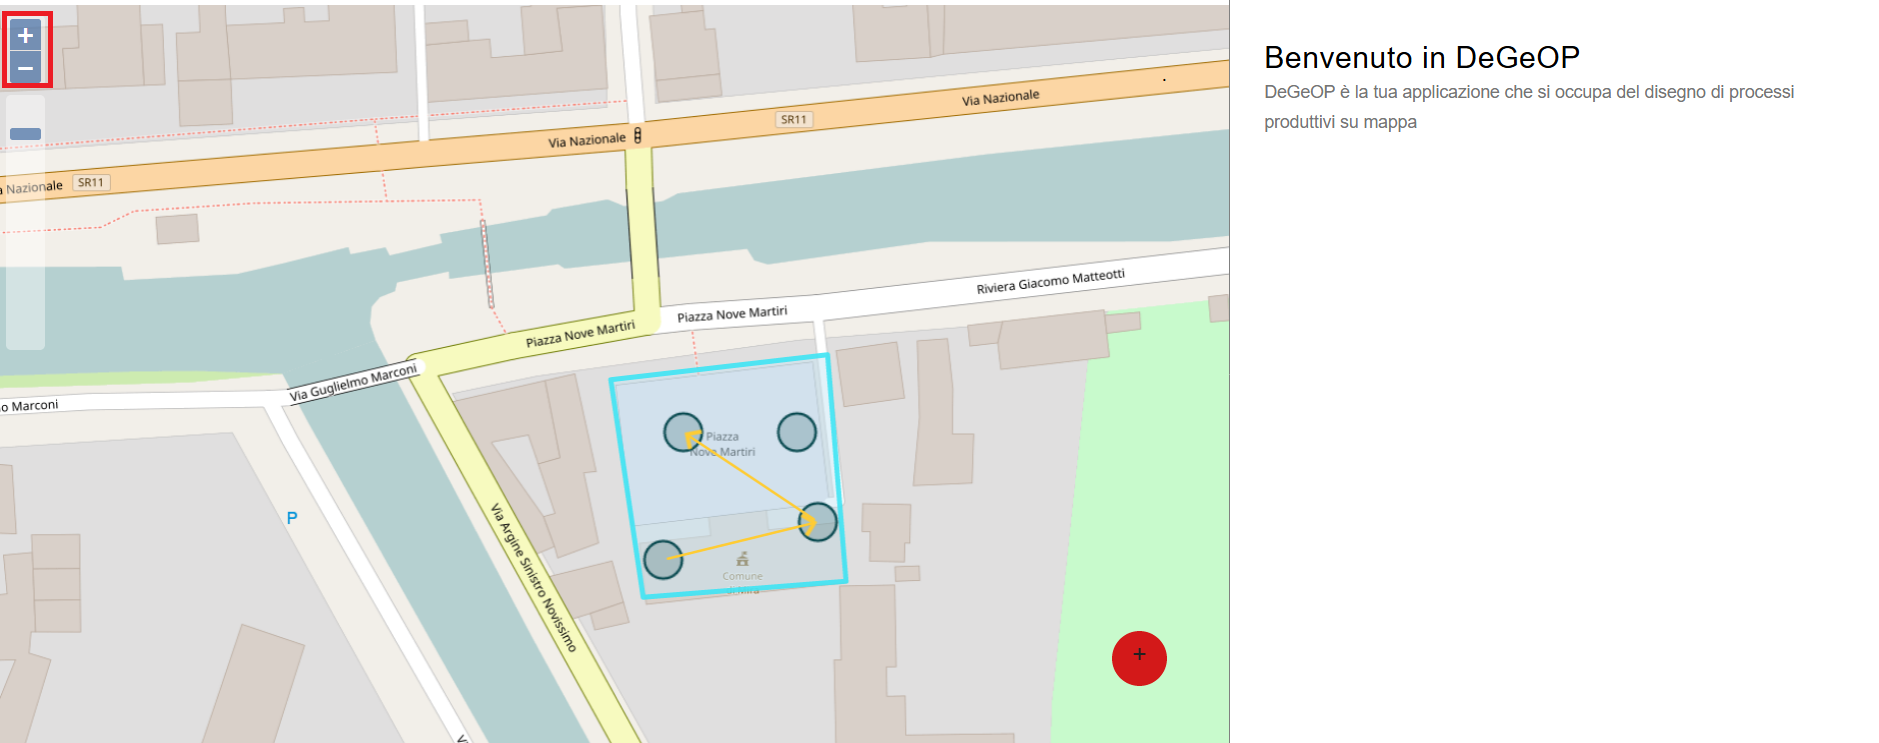
\includegraphics[width=\textwidth]{img/zoom.png}
\caption{Zoom}
\end{figure}

\subsection{Spostarsi sulla mappa}
Per spostarsi sulla mappa è possibile:
\begin{itemize}
	\item spostandosi sulla mappa trascinandola;
	\item utilizzare la \mglo{Gesture}{gesture} "drag" (solo in caso di fruizione da tablet).
\end{itemize}